\documentclass{article}
\usepackage{enumerate}
\usepackage{amsmath}
\usepackage{amssymb}
\usepackage{graphicx}
\usepackage{subfigure}
\usepackage{geometry}
\usepackage{caption}
\usepackage{indentfirst}
\geometry{left=3.0cm,right=3.0cm,top=3.0cm,bottom=4.0cm}
\renewcommand{\thesection}{Problem \arabic{section}.}
%\allowdisplaybreaks[4]
\newcommand{\Omegacm}{{\rm\,\Omega\cdot cm}}
\newcommand{\unit}[1]{{\rm\,#1}}

\title{VE311 Homework 3}
\author{Liu Yihao 515370910207}
\date{}

\begin{document}
\maketitle

\section{}
\begin{enumerate}[(a)]
\item
$$\phi_j=V_T\ln\frac{N_AN_D}{n_i^2}=0.025\unit{V}\cdot\ln\frac{10^{19}\unit{cm^{-3}}\cdot10^{18}\unit{cm^{-3}}}{(10^{10}\unit{cm^{-3}})^2}\approx0.979\unit{V}$$
\begin{align*}
w_{do}&=\sqrt{\frac{2\varepsilon_s}{q}\left(\frac{1}{N_A}+\frac{1}{N_D}\right)\phi_j}\\
&=\sqrt{\frac{2\cdot11.7\cdot8.85\times10^{-14}\unit{F/cm}}{1.60\times10^{-19}\unit{C}}\left(\frac{1}{10^{19}\unit{cm^{-3}}}+\frac{1}{10^{18}\unit{cm^{-3}}}\right)0.979\unit{V}}\\
&\approx3.73\times10^{-2}\unit{\mu m}
\end{align*}
\item
$$x_p=\frac{w_{do}}{1+\dfrac{N_A}{N_D}}=\frac{3.73\times10^{-2}\unit{\mu m}}{1+\dfrac{10^{19}\unit{cm^{-3}}}{10^{18}\unit{cm^{-3}}}}\approx3.39\times10^{-3}\unit{\mu m}$$
$$x_n=\frac{w_{do}}{1+\dfrac{N_D}{N_A}}=\frac{3.73\times10^{-2}\unit{\mu m}}{1+\dfrac{10^{18}\unit{cm^{-3}}}{10^{19}\unit{cm^{-3}}}}\approx3.39\times10^{-2}\unit{\mu m}$$
\item
$$\phi_j=0.979\unit{V}$$
\item
$$E_{MAX}=\frac{qN_Ax_p}{\varepsilon_s}=\frac{1.60\times10^{-19}\unit{C}\cdot10^{19}\unit{cm^{-3}}\cdot3.39\times10^{-3}\unit{\mu m}}{11.7\cdot8.85\times10^{-14}\unit{F/cm}}\approx523\unit{kV/cm}$$
\end{enumerate}

\section{}
\begin{enumerate}[(a)]
\item
$$w_d=w_{do}\sqrt{1+\frac{v_R}{\phi_j}}=3w_{do}$$
$$v_R=8\phi_j=8\cdot0.85\unit{V}=6.8\unit{V}$$
\item
$$w_d=w_{do}\sqrt{1+\frac{v_R}{\phi_j}}=0.4\unit{\mu m}\cdot\sqrt{1+\frac{7\unit{V}}{0.85\unit{V}}}\approx1.22\unit{\mu m}$$
\end{enumerate}

\section{}
$$j=\sigma E$$
$$E=\frac{j}{\sigma}=j\rho=5000\unit{A/cm^2}\cdot2.5\Omegacm=12.5\unit{kV/cm}$$

\section{}
$$p(x)=N_A(x)=N_o\exp\left(-\frac{x}{L}\right)$$
$$j_p^T=qp\mu_pE-qD_p\frac{\partial p}{\partial x}=qp\mu_p\left(E-V_T\frac{1}{p}\frac{\partial p}{\partial x}\right)=0$$
$$E(x)=V_T\frac{1}{p}\frac{\partial p}{\partial x}=\frac{V_T}{N_o\exp\left(-\frac{x}{L}\right)}\cdot-\frac{N_o}{L}\exp\left(-\frac{x}{L}\right)=-\frac{V_T}{L}$$

So a built-in electric field must exist.
$$E=-\frac{V_T}{L}=-\frac{0.025\unit{V}}{1\unit{\mu m}}=-0.25\unit{kV/cm}$$

\section{}
$$nV_T=n\frac{kT}{q}=1.05\cdot\frac{1.38\times10^{-23}\unit{J/K}\cdot320\unit{K}}{1.60\times10^{-19}\unit{C}}\approx0.029\unit{V}$$

If $n=1.00$,
$$nV_T=n\frac{kT}{q}=0.029\unit{V}$$
$$T=\frac{0.029\unit{V}\cdot q}{k}=\frac{0.029\unit{V}\cdot1.60\times10^{-19}\unit{C}}{1.38\times10^{-23}\unit{J/K}}\approx336\unit{K}$$

\section{}
\begin{enumerate}[(a)]
\item
$$V_D=nV_T\ln\left(1+\frac{I_D}{I_S}\right)=1.07\cdot0.025\unit{V}\cdot\ln\left(1+\frac{70\unit{\mu A}}{10^{-17}\unit{A}}\right)\approx0.791\unit{V}$$
\item
$$V_D=nV_T\ln\left(1+\frac{I_D}{I_S}\right)=1.07\cdot0.025\unit{V}\cdot\ln\left(1+\frac{5\unit{\mu A}}{10^{-17}\unit{A}}\right)\approx0.721\unit{V}$$
\item
$$I_D=I_S\left[\exp\left(\frac{V_D}{nV_T}\right)-1\right]=10^{-17}\unit{A}\cdot\left[\exp\left(\frac{0}{1.07\cdot0.025\unit{V}}\right)-1\right]=0\unit{A}$$
\item
$$I_D=I_S\left[\exp\left(\frac{V_D}{nV_T}\right)-1\right]=10^{-17}\unit{A}\cdot\left[\exp\left(\frac{-0.075\unit{V}}{1.07\cdot0.025\unit{V}}\right)-1\right]\approx-9.39\times10^{-18}\unit{A}$$
\item
$$I_D=I_S\left[\exp\left(\frac{V_D}{nV_T}\right)-1\right]=10^{-17}\unit{A}\cdot\left[\exp\left(\frac{-5\unit{V}}{1.07\cdot0.025\unit{V}}\right)-1\right]\approx-1.00\times10^{-17}\unit{A}$$
\end{enumerate}

\section{}
$$V_D=V_T\ln\left(1+\frac{I_D}{I_S}\right)$$
$$V_{D,MAX}=V_T\ln\left(1+\frac{I_D}{I_{S,MIN}}\right)=0.025\unit{V}\ln\left(1+\frac{1\unit{mA}}{10^{-14}\unit{A}}\right)\approx0.633\unit{V}$$
$$V_{D,MIN}=V_T\ln\left(1+\frac{I_D}{I_{S,MAX}}\right)=0.025\unit{V}\ln\left(1+\frac{1\unit{mA}}{10^{-12}\unit{A}}\right)\approx0.518\unit{V}$$
$$0.518\unit{V}\leqslant V_D\leqslant0.633\unit{V}$$

\section{}
\begin{enumerate}[(a)]
\item
\begin{align*}
V_D&=V_T\ln\left(1+\frac{I_D}{I_S}\right)=\frac{kT}{q}\ln\left(1+\frac{I_D}{I_S}\right)\\
&=\frac{1.38\times10^{-23}\unit{J/K}\cdot303\unit{K}}{1.60\times10^{-19}\unit{C}}\ln\left(1+\frac{1\unit{mA}}{2.5\times10^{-16}\unit{A}}\right)\\
&\approx0.758\unit{V}
\end{align*}
\item
$$\frac{dV_D}{dT}=\frac{v_D-V_{GO}-3V_T}{T}=-2\unit{mV/K}$$
\begin{align*}
V_D&=T\frac{dV_D}{dT}+V_{GO}+3\frac{kT}{q}\\
&=323\unit{K}\cdot-2\unit{mV/K}+1.12\unit{V}+3\cdot\frac{1.38\times10^{-23}\unit{J/K}\cdot323\unit{K}}{1.60\times10^{-19}\unit{C}}\\
&\approx0.558\unit{V}
\end{align*}
\end{enumerate}

\section{}
$$\phi_j=V_T\ln\frac{N_AN_D}{n_i^2}=0.025\unit{V}\cdot\ln\frac{10^{18}\unit{cm^{-3}}\cdot10^{20}\unit{cm^{-3}}}{(10^{10}\unit{cm^{-3}})^2}\approx1.036\unit{V}$$
\begin{align*}
w_{do}&=\sqrt{\frac{2\varepsilon_s}{q}\left(\frac{1}{N_A}+\frac{1}{N_D}\right)\phi_j}\\
&=\sqrt{\frac{2\cdot11.7\cdot8.85\times10^{-14}\unit{F/cm}}{1.60\times10^{-19}\unit{C}}\left(\frac{1}{10^{18}\unit{cm^{-3}}}+\frac{1}{10^{20}\unit{cm^{-3}}}\right)1.036\unit{V}}\\
&\approx3.68\times10^{-2}\unit{\mu m}
\end{align*}

When $v_R=5\unit{V}$,
$$w_d=w_{do}\sqrt{1+\frac{v_R}{\phi_j}}=3.68\times10^{-2}\unit{\mu m}\cdot\sqrt{1+\frac{5\unit{V}}{1.036\unit{V}}}\approx8.88\times10^{-2}\unit{\mu m}$$

When $v_R=25\unit{V}$,
$$w_d=w_{do}\sqrt{1+\frac{v_R}{\phi_j}}=3.68\times10^{-2}\unit{\mu m}\cdot\sqrt{1+\frac{25\unit{V}}{1.036\unit{V}}}\approx0.184\unit{\mu m}$$

\section{}
\begin{enumerate}[(a)]
\item
$$V_D=0,I_D=10\unit{V}/5\unit{k\Omega}=2\unit{mA}{\rm\quad and\quad}V_D=10\unit{V},I_D=0$$
\begin{center}
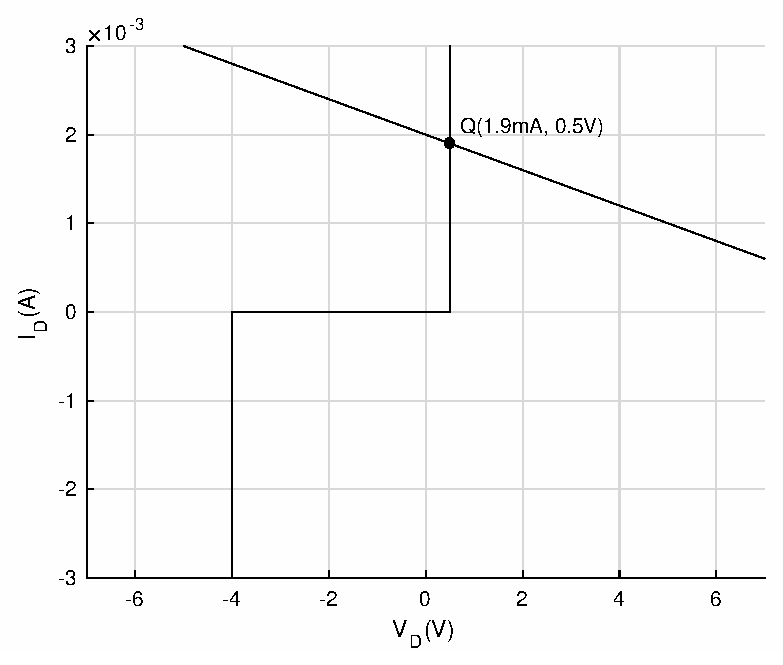
\includegraphics[width=0.5\linewidth]{matlab/iv-1.eps}
\end{center}
\item
$$V_D=0,I_D=-10\unit{V}/5\unit{k\Omega}=-2\unit{mA}{\rm\quad and\quad}V_D=-10\unit{V},I_D=0$$
\begin{center}
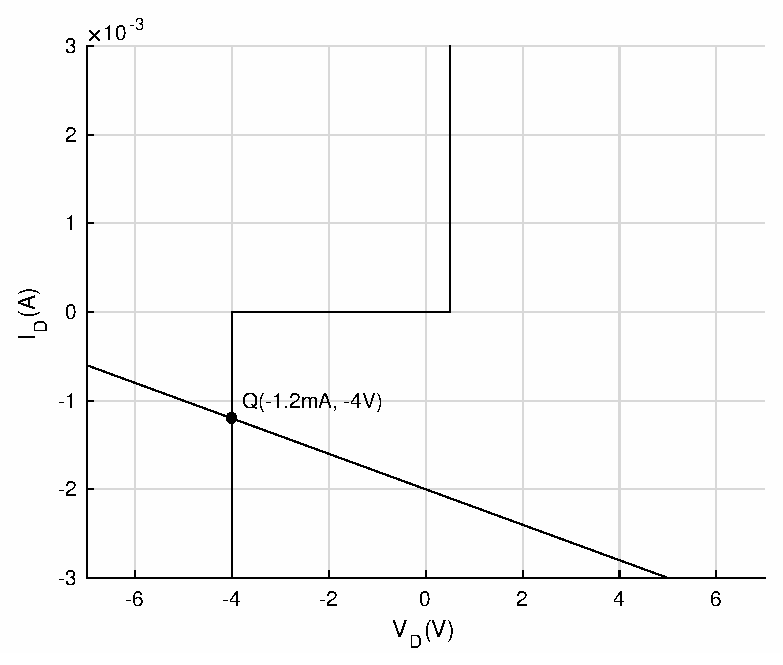
\includegraphics[width=0.5\linewidth]{matlab/iv-2.eps}
\end{center}
\item
$$V_D=0,I_D=-2\unit{V}/2\unit{k\Omega}=-1\unit{mA}{\rm\quad and\quad}V_D=-2\unit{V},I_D=0$$
\begin{center}
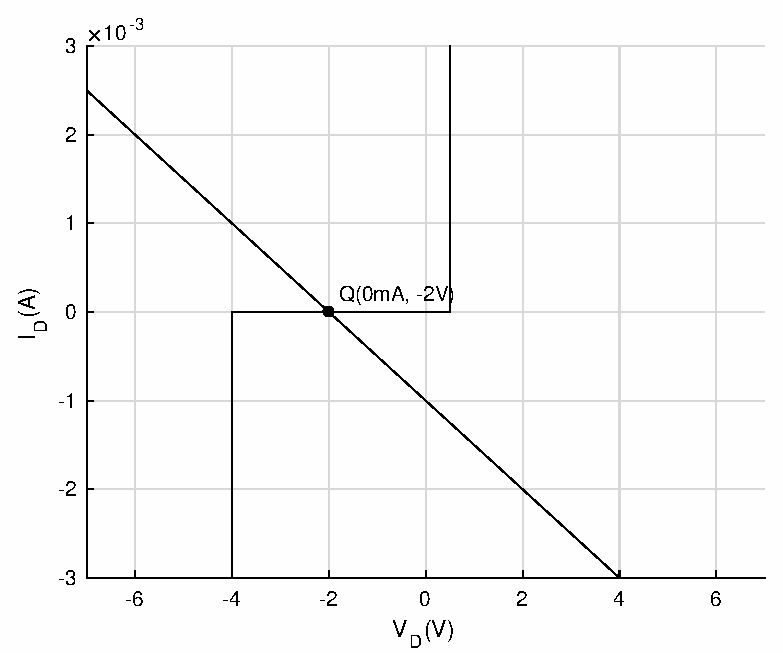
\includegraphics[width=0.5\linewidth]{matlab/iv-3.eps}
\end{center}
\end{enumerate}

\section{}
\begin{enumerate}[(a)]
\item
$$V_D=0,I_D=6\unit{V}/4\unit{k\Omega}=1.5\unit{mA}{\rm\quad and\quad}V_D=6\unit{V},I_D=0$$
\begin{center}
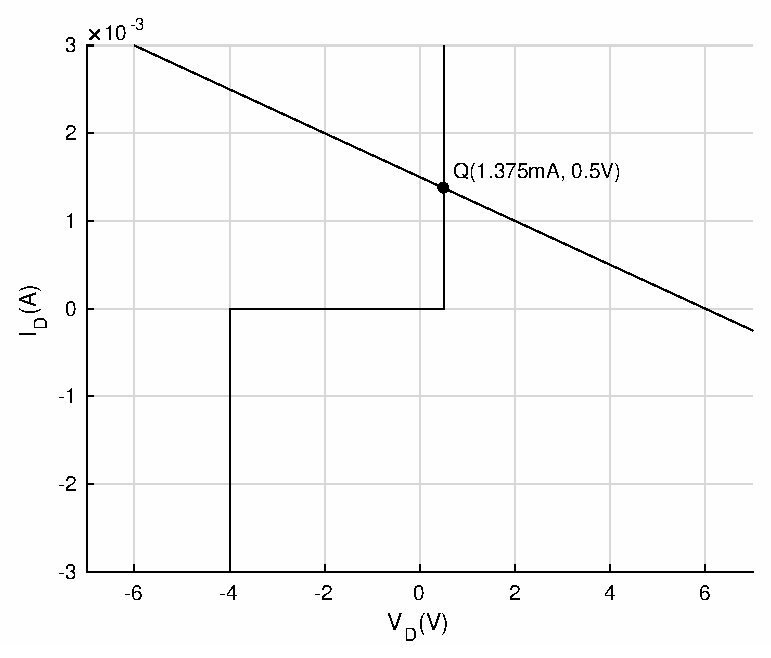
\includegraphics[width=0.5\linewidth]{matlab/iv-4.eps}
\end{center}
\item
$$V_D=0,I_D=-6\unit{V}/3\unit{k\Omega}=-2\unit{mA}{\rm\quad and\quad}V_D=-6\unit{V},I_D=0$$
\begin{center}
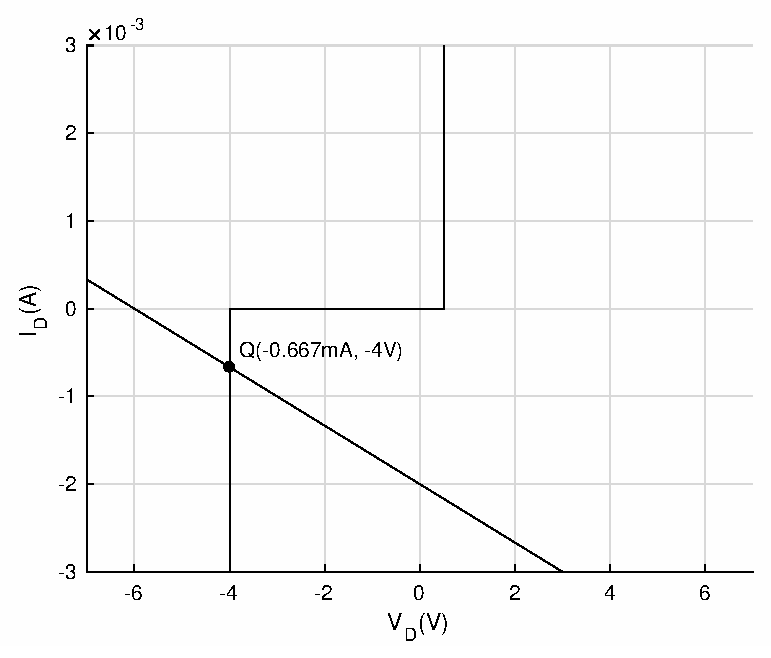
\includegraphics[width=0.5\linewidth]{matlab/iv-5.eps}
\end{center}
\item
$$V_D=0,I_D=-3\unit{V}/3\unit{k\Omega}=-1\unit{mA}{\rm\quad and\quad}V_D=-3\unit{V},I_D=0$$
\begin{center}
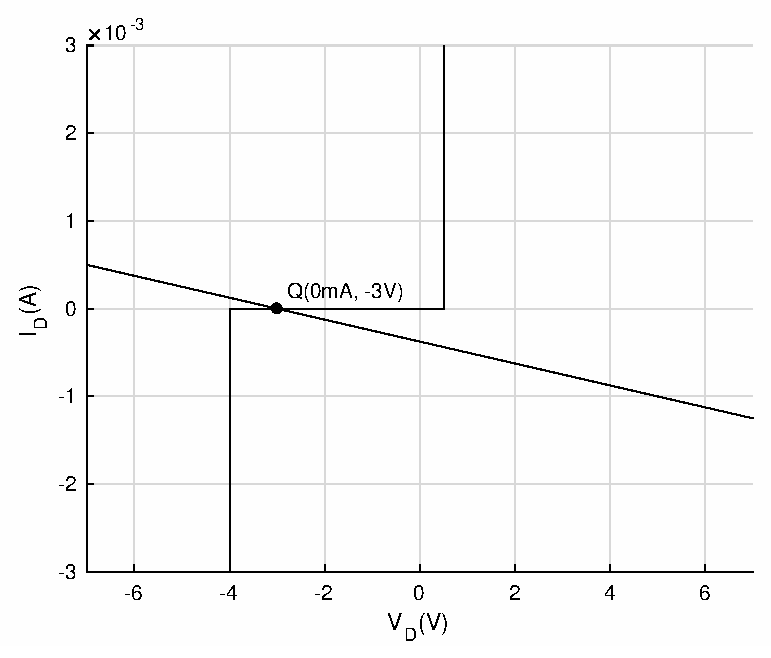
\includegraphics[width=0.5\linewidth]{matlab/iv-6.eps}
\end{center}
\item
$$V_D=0,I_D=12\unit{V}/8\unit{k\Omega}=1.5\unit{mA}{\rm\quad and\quad}V_D=12\unit{V},I_D=0$$
\begin{center}
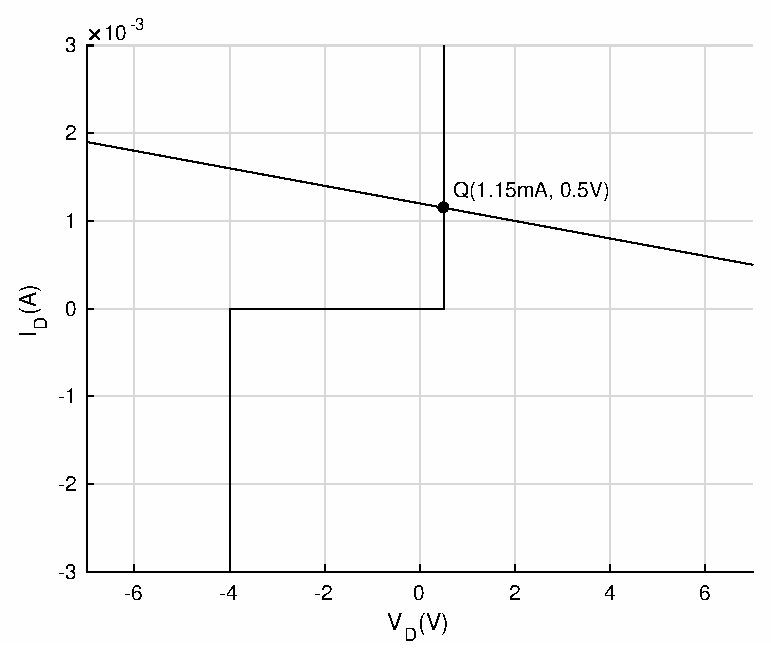
\includegraphics[width=0.5\linewidth]{matlab/iv-7.eps}
\end{center}
\item
$$V_D=0,I_D=-25\unit{V}/10\unit{k\Omega}=-2.5\unit{mA}{\rm\quad and\quad}V_D=-25\unit{V},I_D=0$$
\begin{center}
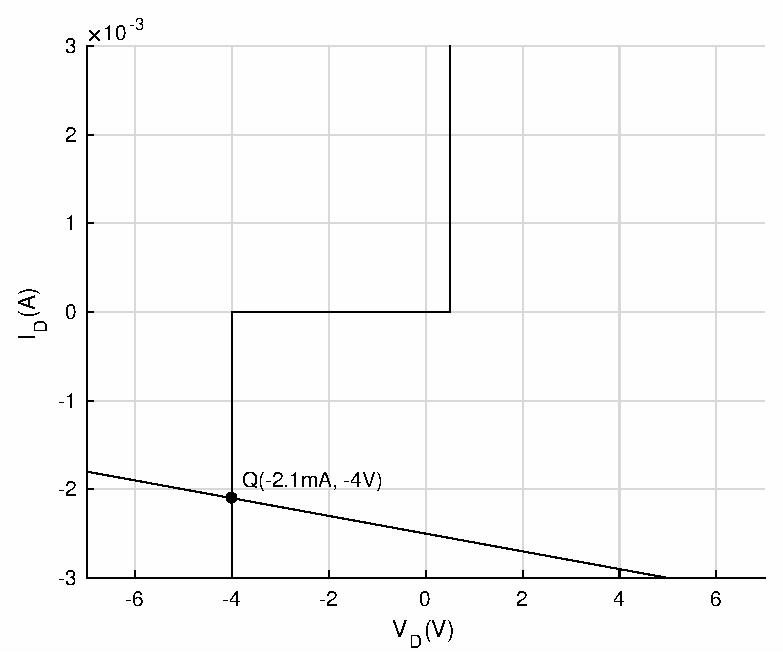
\includegraphics[width=0.5\linewidth]{matlab/iv-8.eps}
\end{center}
\end{enumerate}

\section{}
When $R_S=0$, assuming $V_{on}=1\unit{V}$
$$V_{dc}=-(V_p-V_{on})=-(10\unit{V}-1\unit{V})=-9\unit{V}$$

$$\left\{\begin{aligned}
V_r&=V_{dc}\left[1-\exp\left(-\frac{T-\Delta T}{RC}\right)\right]\\
\Delta T&=\frac{1}{\omega}\sqrt{\frac{2|V_r|}{V_p}}
\end{aligned}\right.\Longrightarrow\left\{\begin{aligned}
V_r&=-6.01\unit{V}\\
\Delta T&=2.91\times10^{-3}\unit{s}
\end{aligned}\right.$$

$$I_P=I_{dc}\frac{2T}{\Delta T}=\frac{2|V_{dc}|T}{R\Delta T}=\frac{2\cdot9\unit{V}\cdot\dfrac{2\pi}{120\pi}\unit{s}}{0.025\unit{\Omega}\cdot2.91\times10^{-3}\unit{s}}\approx4123\unit{A}$$

%When $R_S=0.02\unit{\Omega}$,

\section{}
assuming $V_{on}=1\unit{V}$,
$$V_1=V_p-V_{on}=40\unit{V}-1\unit{V}=39\unit{V}$$
$$V_2=-(V_p-V_{on})=-(40\unit{V}-1\unit{V})=-39\unit{V}$$

\end{document}
|